
\documentclass{beamer} 
% !TeX spellcheck = es_CL

\mode<presentation>
{
  \usetheme{Berkeley}
  % or ...

  \setbeamercovered{transparent}
  % or whatever (possibly just delete it)
}

\usepackage{tikz}
\usepackage{graphicx}
\usepackage[english]{babel}
% or whatever

\usepackage[utf8]{inputenc}
% or whatever

\usepackage{times}
\usepackage[T1]{fontenc}
% Or whatever. Note that the encoding and the font should match. If T1
% does not look nice, try deleting the line with the fontenc.


\title[Transparencia en Investigación en las Ciencias Sociales] % (optional, use only with long paper titles)
{Transparencia en Investigación en las Ciencias Sociales}

\subtitle
{}

\author[Hoces] % (optional, use only with lots of authors)
{Fernando~Hoces de la Guardia\inst{1}}
% - Give the names in the same order as the appear in the paper.
% - Use the \inst{?} command only if the authors have different
%   affiliation.

\institute[Universities of Somewhere and Elsewhere] % (optional, but mostly needed)
{
  \inst{1}%
  UC Berkeley:\\
  Berkeley Initiative for Transparency in the Social Sciences\\
  }
% - Use the \inst command only if there are several affiliations.
% - Keep it simple, no one is interested in your street address.

\date[BITSS2017] % (optional, should be abbreviation of conference name)
{Pontificia Universidad Católica, Octubre 2017\\
Slides disponibles en \url{COMPLETAR}}
% - Either use conference name or its abbreviation.
% - Not really informative to the audience, more for people (including
%   yourself) who are reading the slides online

\subject{Transparencia en Investigación}
% This is only inserted into the PDF information catalog. Can be left
% out. 

\pgfdeclareimage[height=2cm]{university-logo}{../Images/BITSSlogo.png}
\logo{\pgfuseimage{university-logo}}

% If you have a file called "university-logo-filename.xxx", where xxx
% is a graphic format that can be processed by latex or pdflatex,
% resp., then you can add a logo as follows:

% \pgfdeclareimage[height=0.5cm]{university-logo}{university-logo-filename}
% \logo{\pgfuseimage{university-logo}}



% Delete this, if you do not want the table of contents to pop up at
% the beginning of each subsection:
%\AtBeginSubsection[]
%{
%  \begin{frame}<beamer>{Outline}
%    \tableofcontents[currentsection,currentsubsection]
%  \end{frame}
%}


% If you wish to uncover everything in a step-wise fashion, uncomment
% the following command: 

\beamerdefaultoverlayspecification{<.->}


\begin{document}

\begin{frame}
  \titlepage
\end{frame}




% Structuring a talk is a difficult task and the following structure
% may not be suitable. Here are some rules that apply for this
% solution: 

% - Exactly two or three sections (other than the summary).
% - At *most* three subsections per section.
% - Talk about 30s to 2min per frame. So there should be between about
%   15 and 30 frames, all told.

% - A conference audience is likely to know very little of what you
%   are going to talk about. So *simplify*!
% - In a 20min talk, getting the main ideas across is hard
%   enough. Leave out details, even if it means being less precise than
%   you think necessary.
% - If you omit details that are vital to the proof/implementation,
%   just say so once. Everybody will be happy with that.
%%%%%%%%%%%%%%%%%%%%%%%%%%%%%%%%%%%%%%%%%%%%%%%%%%%%%%%%%%%%%%%%%%%%%%%
%%%%%%%%%%%%%%%%%%%%%%%%%%%%%%%%%%%%%%%%%%%%%%%%%%%%%%%%%%%%%%%%%%%%%
\begin{frame}
Primero, un favor: ¿Podrían completar esta breve encuesta [en ingles]?

\huge{\url{https://goo.gl/0yIhEu}}


\end{frame}

\begin{frame}{Estructura de la Presentación}
  \tableofcontents
  % You might wish to add the option [pausesections]
\end{frame}

\section {Introducción}
{ % all template changes are local to this group.
    \setbeamertemplate{navigation symbols}{}
    \begin{frame}[plain]
        \begin{tikzpicture}[remember picture,overlay]
            \node[at=(current page.center)] {
                \href{https://www.bitss.org/}{
\includegraphics[width=\paperwidth]{../Images/BITSSlogo.png}}
            };
        \end{tikzpicture}
     \end{frame}
}

{ % all template changes are local to this group.
    \setbeamertemplate{navigation symbols}{}
    \begin{frame}[plain]
        \begin{tikzpicture}[remember picture,overlay]
            \node[at=(current page.center)] {
                \href{https://www.bitss.org/}{
\includegraphics[width=\paperwidth]{../Images/ecosystem.PNG}}
            };
        \end{tikzpicture}
     \end{frame}
}
%%%%%%%%%%%%%%%%%%%%%%%%%%%%%%%%%%%%%%%%%%%%%%%%%%%%%%%%%%%%%%%%%%%%%%%%%%%%%%%%%%%
\section{Ética en la Investigación Científica}
\begin{frame}{Ética en la Investigación Científica}
\begin{itemize}
\item Transparencia es un elemento central de la ética del investigador.

\item Valores científicos acuñados por Robert Merton (Merton 1942):
\begin{itemize}[<.->]
\item Universalismo: cualquier persona puede presentar un argumento, independiente de su estatus.
\item Comunismo: el conocimiento es compartido de manera abierta.
\item Desinterés: la verdad como motivación, y no los beneficios monetarios.
\item Escepticismo Organizado: revisión a través de pares (peer review), replicación.
\end{itemize}
\end{itemize}
\end{frame}

\begin{frame}{Ética en la Investigación Científica}
\begin{itemize}
\item
Casos de fraude existen \href{http://pss.sagepub.com/content/24/10/1875}{(Simonsohn 2013)}, pero más importante como investigadores tenemos que admitir nuestra condicion humana, sujeto as sesgos y razonamiento motivado, transparencia puede ayudar con esto \href{http://pps.sagepub.com/content/7/6/615.short}{(Nosek, Spies, Motyl 2012)}.
\item
Quienes llevamos a cabo experimentos o usamos datos con información identificable a nivel individual, tenemos que tomar con seriedad los Comités de Ética Institucionales (IRBs) (Ch. 11--13 Morton \& Williams 2010, \href{http://desposato.org/ethicsfieldexperiments.pdf}{Desposato 2014}). 
\end{itemize}
\end{frame}

%{ % all template changes are local to this group.
%    \setbeamertemplate{navigation symbols}{}
%    \begin{frame}[plain]
%        \begin{tikzpicture}[remember picture,overlay]
%            \node[at=(current page.center)] {
%                
\includegraphics[height=\paperheight]{../Images/motivatedreasoning.PNG}
%            };
%        \end{tikzpicture}
%     \end{frame}
%}
%{ % all template changes are local to this group.
%    \setbeamertemplate{navigation symbols}{}
%    \begin{frame}[plain]
%        \begin{tikzpicture}[remember picture,overlay]
%            \node[at=(current page.center)] {
%                \href{http://www.nytimes.com/2014/10/29/upshot/professors-research-project-%stirs-political-outrage-in-montana.html}{
\includegraphics[width=\paperwidth]{../Images/Montana1.PNG}}
%            };
%        \end{tikzpicture}
%     \end{frame}
%}
%{ % all template changes are local to this group.
%    \setbeamertemplate{navigation symbols}{}
%    \begin{frame}[plain]
%        \begin{tikzpicture}[remember picture,overlay]
%            \node[at=(current page.center)] {
%                \href{https://www.washingtonpost.com/news/monkey-cage/wp/2015/05/13/campaign-experiment-found-to-be-in-violation-of-montana-law/}{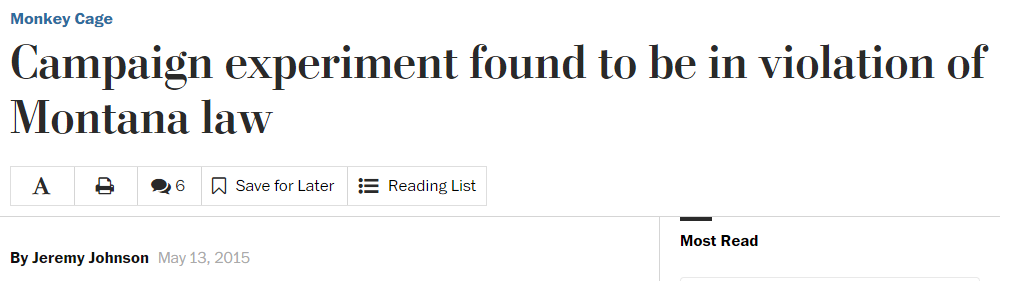
\includegraphics[width=\paperwidth]{../Images/Montana2.PNG}}
%            };
%        \end{tikzpicture}
%     \end{frame}
%}

%HERE'S THE BASIC SYNTAX TO SHOW FIGURE AND IMAGE ON SAME SLIDE
%\begin{frame}
%Why we worry: \href{http://pss.sagepub.com/content/23/5/524}{(John, Loewenstein, Prelec 2011)}
%\frame{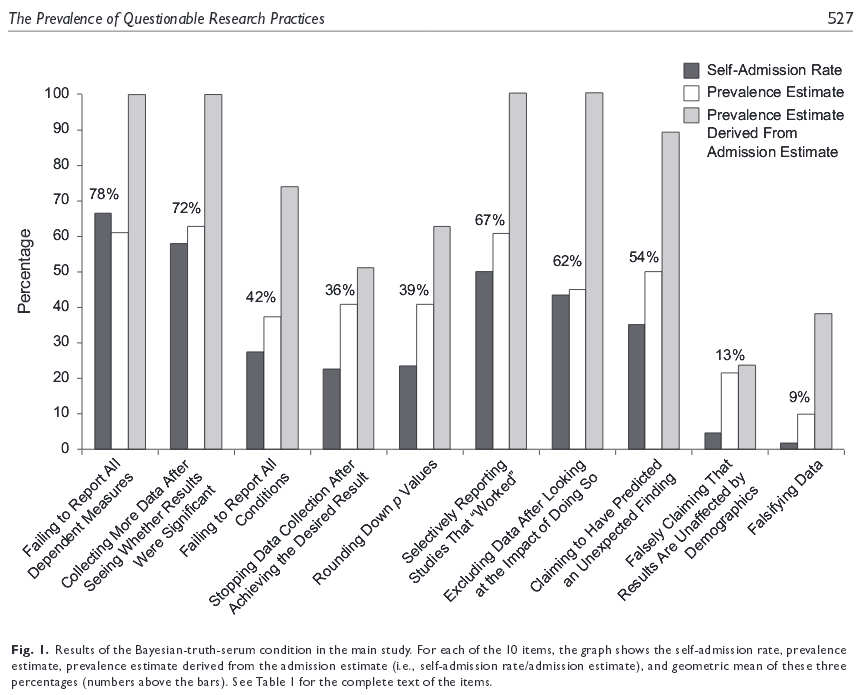
\includegraphics[scale=0.375]{../Images/PrelecFig1.PNG}}
%\end{frame}

\begin{frame}{Ética en la Investigación Científica}
Por que nos preocupamos:
\begin{itemize}[<.->]
\item \href{http://www.jstor.org/stable/pdf/10.1525/jer.2007.2.4.3.pdf}{(Anderson, Martinson, De Vries 2007)}
\item \href{http://pss.sagepub.com/content/23/5/524}{(John, Loewenstein, Prelec 2011)}
\end{itemize}
\end{frame}

{ % all template changes are local to this group.
    \setbeamertemplate{navigation symbols}{}
    \begin{frame}[plain]
        \begin{tikzpicture}[remember picture,overlay]
            \node[at=(current page.center)] {
                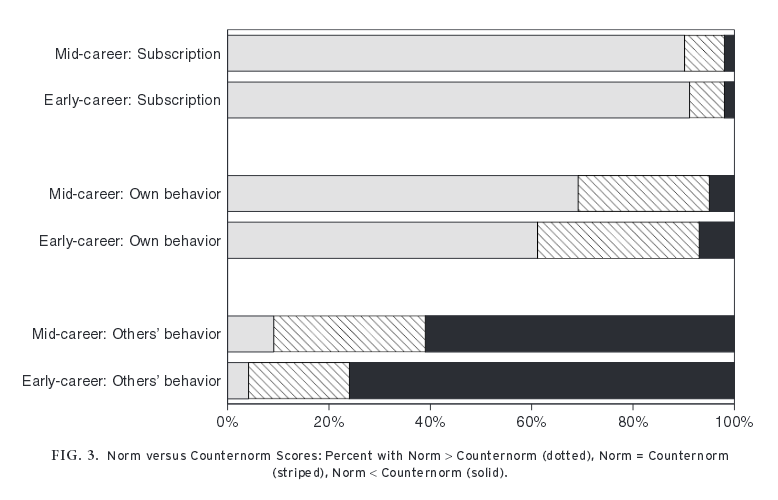
\includegraphics[width=\paperwidth]{../Images/AMdV2007.PNG}
            };
        \end{tikzpicture}
     \end{frame}
}
{ % all template changes are local to this group.
    \setbeamertemplate{navigation symbols}{}
    \begin{frame}[plain]
        \begin{tikzpicture}[remember picture,overlay]
            \node[at=(current page.center)] {
                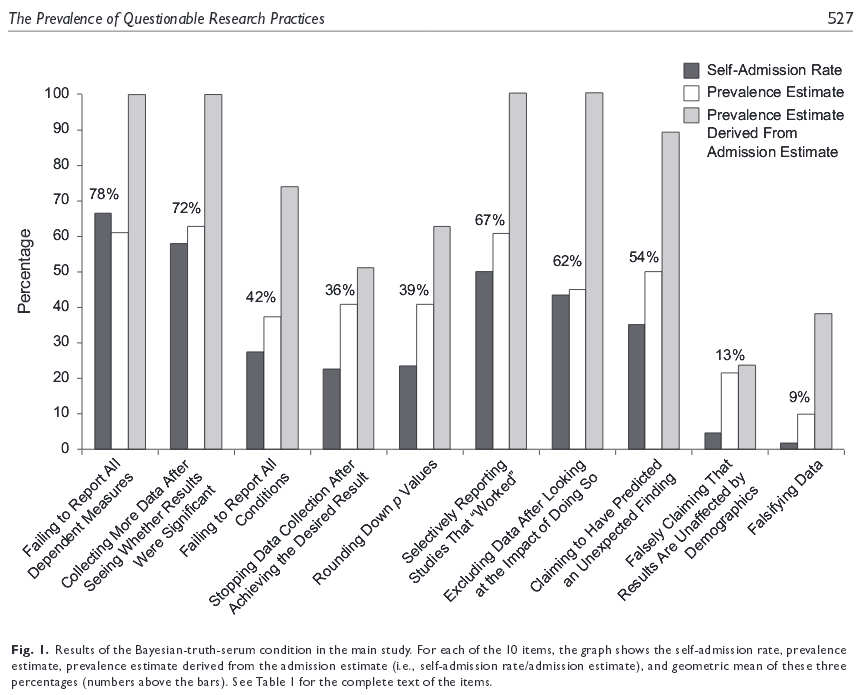
\includegraphics[height=\paperheight]{../Images/PrelecFig1.PNG}
            };
        \end{tikzpicture}
     \end{frame}
}

%\end{frame}
%%%%%%%%%%%%%%%%%%%%%%%%%%%%%%%%%%%%%%%%%%%%%%%%%%%%%%%%%%%%%%%%%%
%\section{Study Design and Power}
%\begin{frame}{Study Design and Power}
%\begin{itemize}[<.->]
%\item
%Adequately power trials to help prevent spurious significant results. 
%\item
%Practical suggestions:
%\begin{itemize}
%\item
%Collaborate with other labs to mutually run each others' experiments (Open Science Collaboration 2014, 2015).
%\begin{itemize}[<.->]
%\item \href{http://science.sciencemag.org/content/349/6251/aac4716.full}{Replication Project: Psychology}
%\item \href{http://econtent.hogrefe.com/doi/full/10.1027/1864-9335/a000178}{Many Labs 1}, \href{https://osf.io/8cd4r/}{2}, 3
%\item Crowdsourcing Analysis \href{http://www.nature.com/news/crowdsourced-research-many-hands-make-tight-work-1.18508}{(Silberzahn and Uhlmann 2016)}
%\item \href{http://science.sciencemag.org/content/early/2016/03/02/science.aaf0918}{Experimental economics replications (Camerer et al. 2016)}
%\end{itemize}
%\item
%Maximize power subject to budget constraint by adjusting expensive treatment arm (relative) size \href{http://citeseerx.ist.psu.edu/viewdoc/download?doi=10.1.1.650.9734&rep=rep1&type=pdf}{(Duflo, Glennerster, Kremer 2007)}. 
%\end{itemize}
%\end{itemize}
%\end{frame}

%{ % all template changes are local to this group.
%    \setbeamertemplate{navigation symbols}{}
%    \begin{frame}[plain]
%        \begin{tikzpicture}[remember picture,overlay]
%            \node[at=(current page.center)] {
%                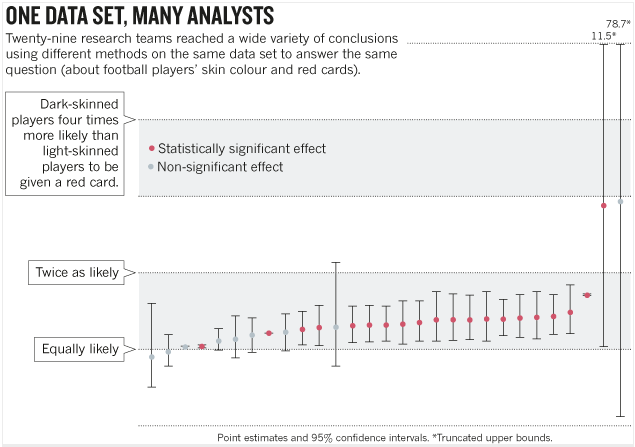
\includegraphics[width=\paperwidth]{../Images/Crowdsourcing2.PNG}
%            };
%        \end{tikzpicture}
%     \end{frame}
%}
%%%%%%%%%%%%%%%%%%%%%%%%%%%%%%%%%%%%%%%%%%%%%%%%%%%%%%%%%%%%%%%%%%%%%
\section{Registros}

\subsection*{Sesgo de Publicación}
\begin{frame}{Sesgo de Publicación}%{Subtitles are optional.}
  % - A title should summarize the slide in an understandable fashion
  %   for anyone how does not follow everything on the slide itself.
  Existencia del problema:
  \begin{itemize}
  \item
 El tamaño de los efectos disminuye con el tamaño muestral (\href{http://pan.oxfordjournals.org/content/9/4/385.short}{Gerber, Green, Nickerson 2001})
  \item
  Las Ciencias Sociales muestran una tasa de rechazo de la hipótesis nula mayor que las ciencias duras (\href{http://journals.plos.org/plosone/article?id=10.1371/journal.pone.0010068}{Fanelli 2010}).
  \item
  La publicación de efectos nulos esta desapareciendo en el tiempo, en todas las disciplinas. (\href{http://link.springer.com/article/10.1007/s11192-011-0494-7}{Fanelli 2011}). 
  \item
  Estudio que  siguió a experimentos completados muestra que aquellos experimentos con fuertes resultados son 40pp más probable de ser publicados, y 60pp más probable de ser escritos. Alto ``file drawer problem''. (\href{http://science.sciencemag.org/content/345/6203/1502}{Franco, Malhotra, Simonovits 2014})
  \end{itemize}
\end{frame}

%Go through the fields

\begin{frame}{Problema en todas las disciplinas}
\begin{itemize}[<.->]
\item Medicina: \href{http://www.nejm.org/doi/full/10.1056/nejmsa065779}{(Turner et al. 2008)}
\item Ciencias Sociales: \href{http://science.sciencemag.org/content/345/6203/1502.short}{(Franco, Malhotra, Simonovits 2014)}
\item Economía: \href{https://www.aeaweb.org/articles.php?doi=10.1257/app.20150044}{(Brodeur et al. 2016)}
\item Sociología: \href{http://smr.sagepub.com/content/37/1/3.short}{(Gerber and Malhotra 2008)}
\item Ciencias Políticas: \href{http://nowpublishers.com/article/Details/QJPS-8024}{(Gerber and Malhotra 2008)}
\end{itemize}
\end{frame}

{ % all template changes are local to this group.
    \setbeamertemplate{navigation symbols}{}
    \begin{frame}[plain]
        \begin{tikzpicture}[remember picture,overlay]
            \node[at=(current page.center)] {
                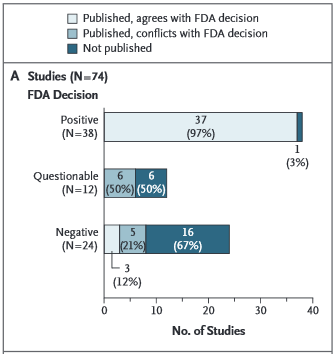
\includegraphics[height=\paperheight]{../Images/TurnerFigure1.PNG}
            };
        \end{tikzpicture}
     \end{frame}
}
{ % all template changes are local to this group.
    \setbeamertemplate{navigation symbols}{}
    \begin{frame}[plain]
        \begin{tikzpicture}[remember picture,overlay]
            \node[at=(current page.center)] {
                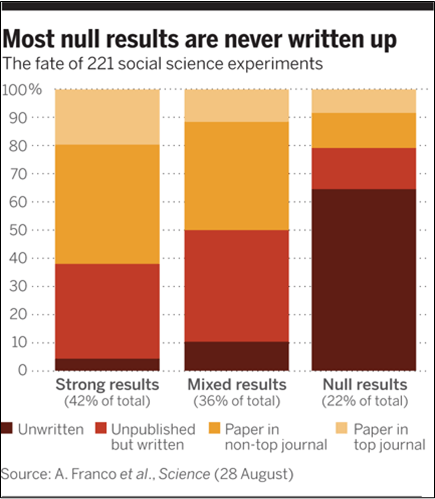
\includegraphics[height=\paperheight]{../Images/Tess.PNG}
            };
        \end{tikzpicture}
     \end{frame}
}
{ % all template changes are local to this group.
    \setbeamertemplate{navigation symbols}{}
    \begin{frame}[plain]
        \begin{tikzpicture}[remember picture,overlay]
            \node[at=(current page.center)] {
                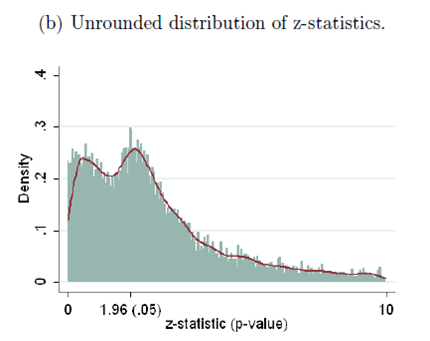
\includegraphics[height=\paperheight]{../Images/Brodeur.PNG}
            };
        \end{tikzpicture}
     \end{frame}
}
{ % all template changes are local to this group.
    \setbeamertemplate{navigation symbols}{}
    \begin{frame}[plain]
        \begin{tikzpicture}[remember picture,overlay]
            \node[at=(current page.center)] {
                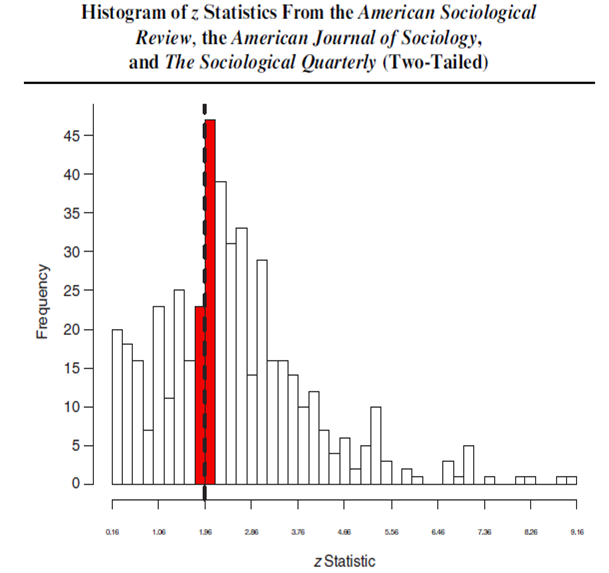
\includegraphics[height=\paperheight]{../Images/GerberSoc.PNG}
            };
        \end{tikzpicture}
     \end{frame}
}
{ % all template changes are local to this group.
    \setbeamertemplate{navigation symbols}{}
    \begin{frame}[plain]
        \begin{tikzpicture}[remember picture,overlay]
            \node[at=(current page.center)] {
                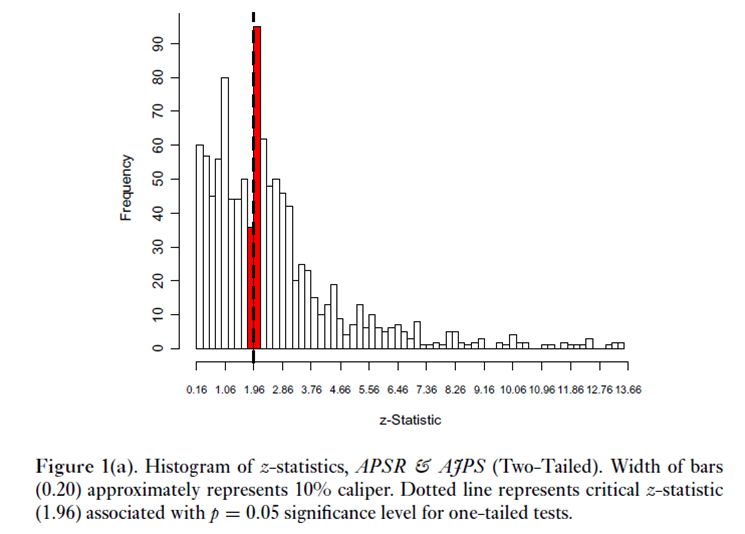
\includegraphics[height=\paperheight]{../Images/GerberPS.PNG}
            };
        \end{tikzpicture}
     \end{frame}
}




\begin {frame}{Sesgo de Publicación}
Si solo escribimos/publicamos resultados significativos, y no dejamos registro de los no significativos, no tenemos forma de distinguir si nuestros resultados ``significativos'' son reales, o si son el 5\% que deberíamos esperar debido a error estadístico. 

%If we only write up/publish significant results, and we have no record of all the insignificant results, we have no way to tell if our `significant' results are real, or if they're the 5\% we should expect due to noise.
\end{frame}

\subsection* {Registros}
\begin{frame}{Registros}
Pre-Registros como una solución al sesgo de publicación:
 \begin{itemize}
  \item
  Hacer publica la investigación a ejecutar, publicando por adelantado las hipótesis a testear.
   %\item If we know every hypothesis test that is run on a given subject, we have a better idea of how seriously to take the significant results.
  \item

   Adopción casi universal en RCTs en medicina. Journals top (ICMJE) no publican estudios si no están registrados. \url{http://clinicaltrials.gov}
   
%  \item
  
%   Even better if registry requires outcomes from after study. Currently limited, but NIH is moving on this.
\end{itemize}
\end{frame}

\begin{frame}{Registros}
Nuevos en ciencias sociales, pero: 
   \begin{itemize}[<.->]
   \item   	
   	Registro de AEA , actualmente solo para RCTs. \url{http://socialscienceregistry.org}
   \item
    Registro de EGAP  \url{http://egap.org/design-registration}
   \item 
    Registro de 3ie, para evaluaciones en países en desarrollo. \url{http://ridie.3ieimpact.org}
   \item
   	Open Science Framework\\ \url{http://osf.io}
   	\begin{itemize}
   	\item
   	Formato abierto
   	\item
   	Pronto va a estar sincronizado con los de más arriba
   	\end{itemize}
   	\item Simple: \url{http://aspredicted.org}
   \end{itemize}
 
\end{frame}

 { % all template changes are local to this group.
    \setbeamertemplate{navigation symbols}{}
    \begin{frame}[plain, label=AEAreg]
         \begin{tikzpicture}[remember picture,overlay]
            \node[at=(current page.center)] {
                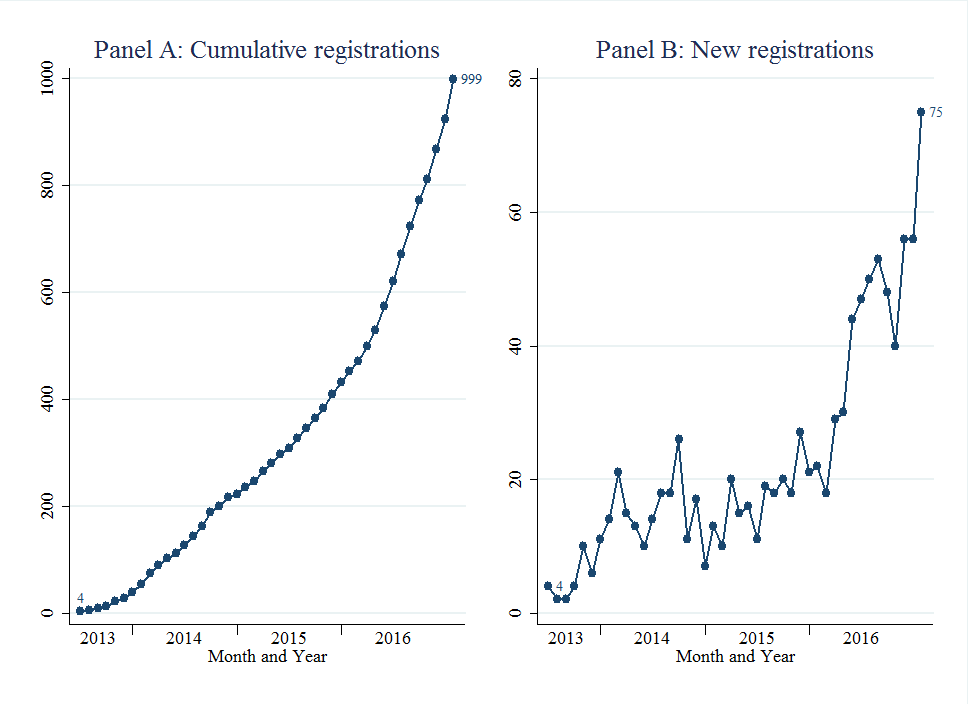
\includegraphics[height=\paperheight]{../Images/combinedAEARegGraphs.png}
            };
        \end{tikzpicture}
     \end{frame}
}

\begin{frame}{Publicaciones Basadas en Diseño de la Investigación}
Alias Reportes Registrados, cambia momento de peer review hacia antes del la recolección de dates, análisis y resultados. 

\begin{enumerate}[<.->]
\item Diseñar un estudio
\item Enviar a un journal
\item Revisión basada en la importancia de la pregunta y calidad del diseño
\item Obtener aceptación en principio
\item Ejecutar el estudio, y publicar incluso con resultados nulos
\end{enumerate}
\href{https://osf.io/8mpji/wiki/home/}{20 Journals, 5 más con con ediciones especiales \beamergotobutton{Link}}
\end{frame}

{ % all template changes are local to this group.
    \setbeamertemplate{navigation symbols}{}
    \begin{frame}[plain, label=AEAreg]
         \begin{tikzpicture}[remember picture,overlay]
            \node[at=(current page.center)] {
                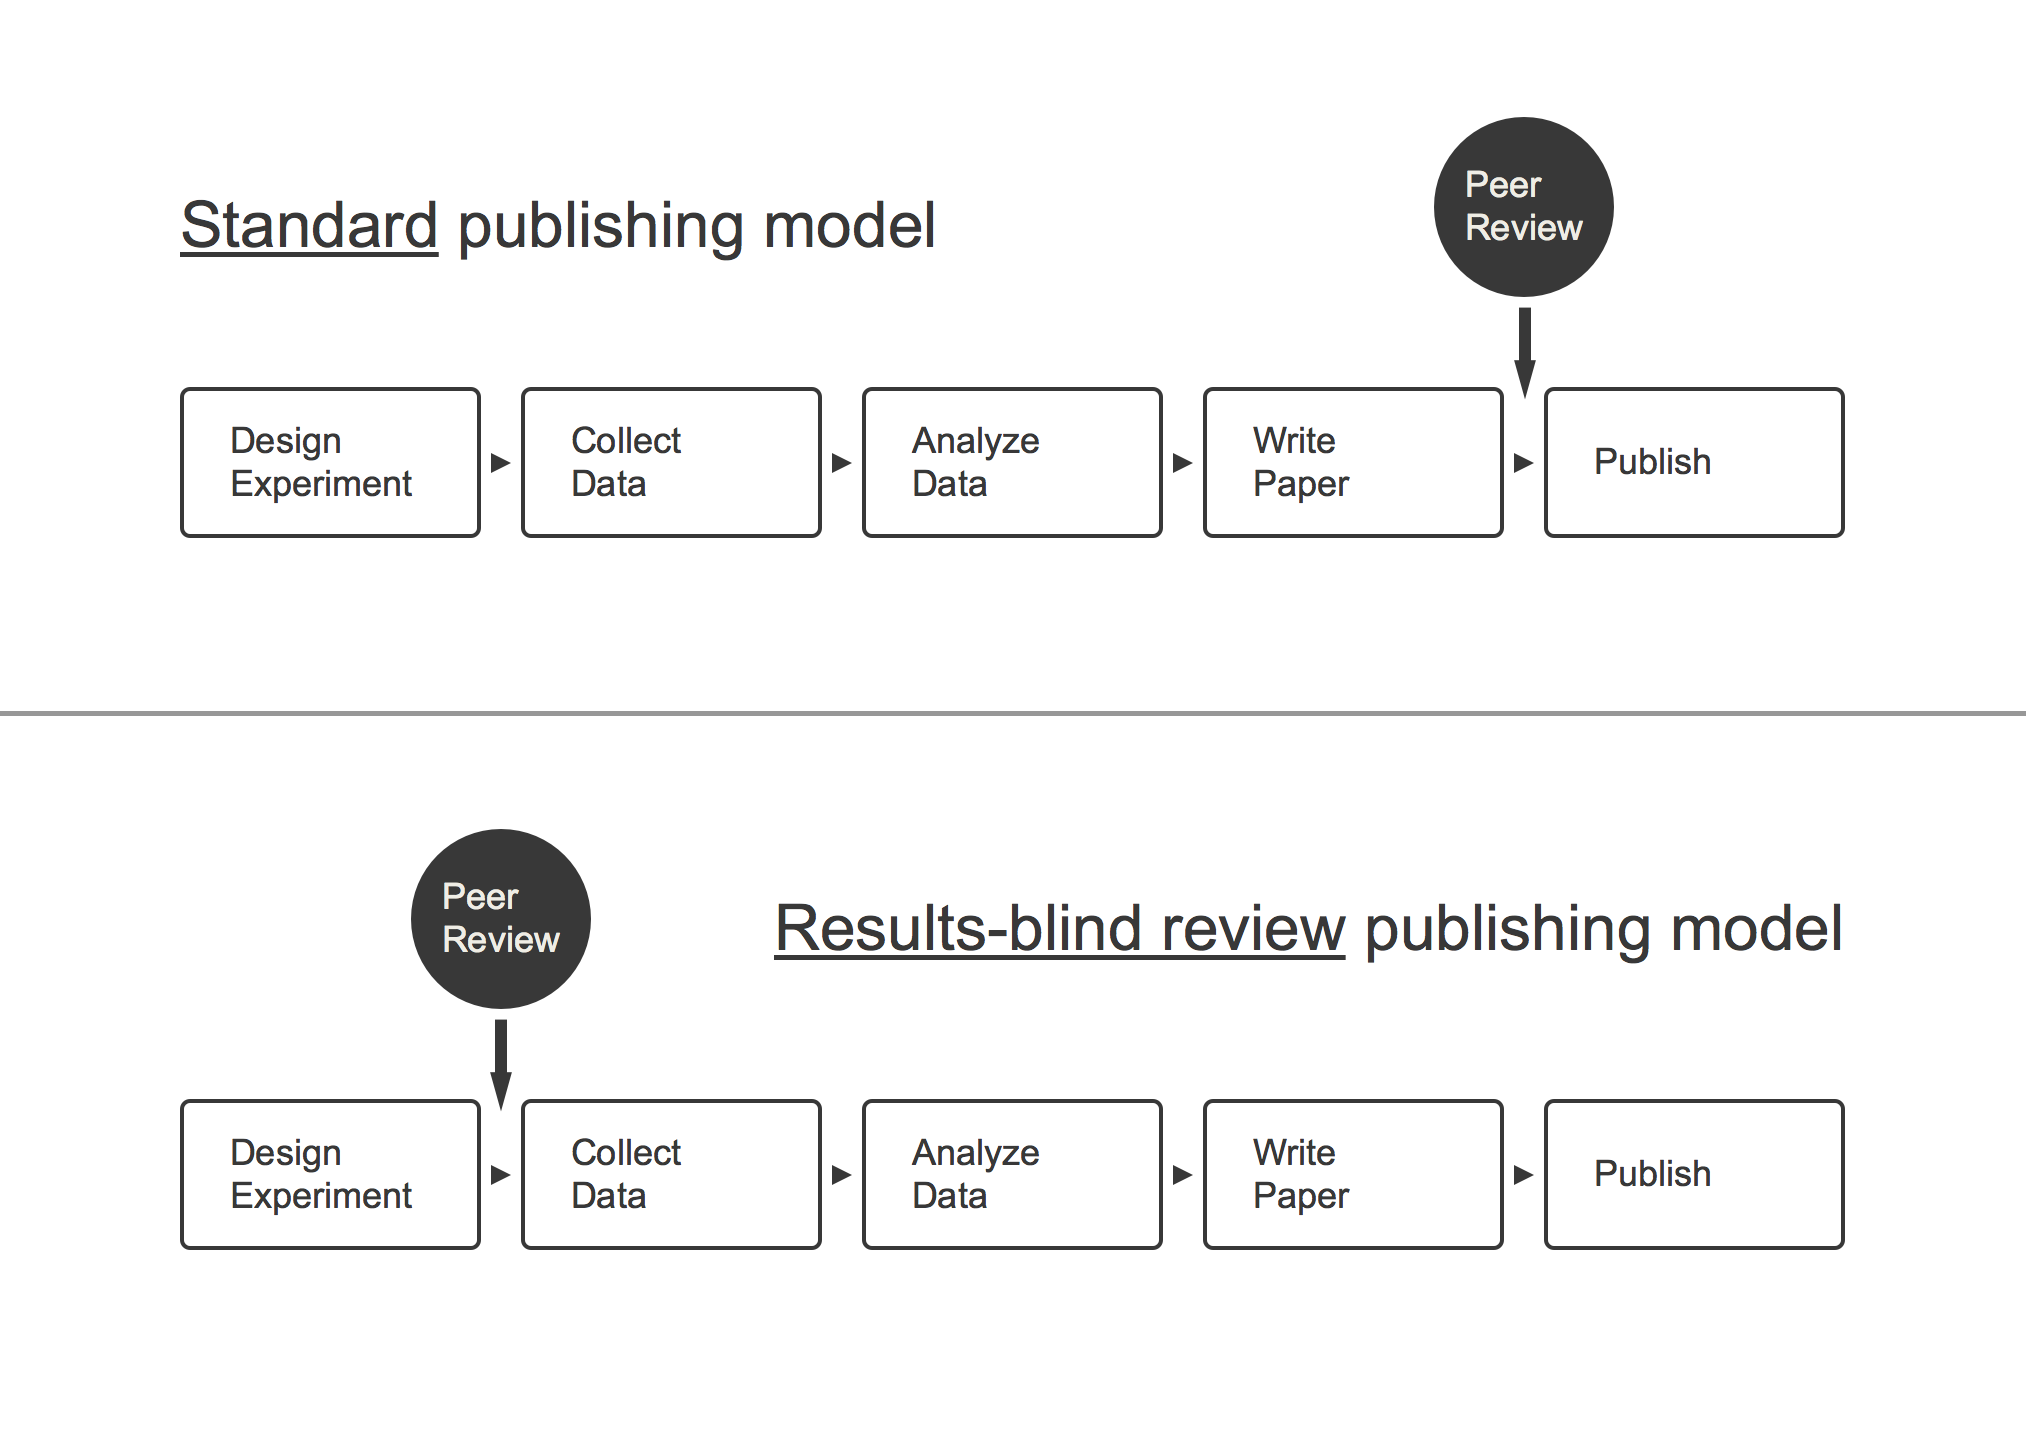
\includegraphics[height=\paperheight]{../Images/results_blind_review.png}
            };
        \end{tikzpicture}
     \end{frame}
}

\begin{frame}{Meta-Análisis}
Síntesis sistemático de los resultados

\vspace{.2in}
Organizaciones:
\begin{itemize}[<.->]
\item Cochrane Collaboration (Medicina)
\item Campbell Collaboration (Políticas Publicas)
\item \href{http://ies.ed.gov/ncee/wwc/}{What Works Clearinghouse (Educación, Gob. US)}
\item \href{http://clear.dol.gov/}{CLEAR (Empleo, Gob. US)}
\item \href{https://www.hendrix.edu/maer-network/}{MAER-NET} (Economía)
\end{itemize}
\end{frame}

\begin{frame}{Meta-Análisis}
Herramientas:
\begin{itemize}[<.->]
\item Funnel plots del tamaño de la muestra vs. tamaño del efecto  \href{http://www.jstor.org/stable/2117925}{(Card \& Krueger 1995)}
\item Funnel Asymmetry Test \href{https://books.google.com/books?id=jSQEdEsL7VoC}{(Stanley \& Doucouliagos 2012)}
\item P-curve \href{http://p-curve.com/}{(Simonsohn et al. 2014)} \href{http://p-curve.com/}{\beamergotobutton{Online App}}
\begin{itemize}
	\item Un p-checker para todos \href{http://shinyapps.org/apps/p-checker/}{\beamergotobutton{Shiny App}}	
\end{itemize}
\end{itemize}
\end{frame}
%%%%%%%%%%%%%%%%%%%%%%%%%%%%%%%%%%%%%%%%%%%%%%%%%%%%%%%%%%%%%%%%%%%%%%%
\section{Pre-Analysis Plans}
\subsection*{P-Hacking}
\begin{frame}[<.->]{P-Hacking}
Definición del problema:
\begin{itemize}
\item
Otros nombres: ``fishing'', grados de libertad del investigador, o ``data-mining''.
\item
Definición: flexibilidad en el análisis de datos permite presentar \textit{casi cualquier resultado} bajo un umbral arbitrario; significancia estadística pierde sentido.
\item
No es algo único de investigadores con malas intenciones. Es subconsciente, o simplemente una practica estándar del análisis estadístico (\href{http://www.stat.columbia.edu/~gelman/research/unpublished/p_hacking.pdf}{Gelman, Loken 2013}).
\end{itemize}
\end{frame}

\begin{frame}{P-Hacking: hágalo usted mismo!}
\begin{itemize}
\item
``Science isn't Broken'' ---538 reportaje periodístico con modulo interactivo \href{http://fivethirtyeight.com/features/science-isnt-broken}{\beamerbutton{Link}}
\item 
Practique p-hacking en R/Shiny App. \href{http://www.nicebread.de/introducing-p-hacker/}{\beamerbutton{Link}}
\item
El Exact Fishy Test \href{https://macartan.shinyapps.io/fish/}{\beamerbutton{Link}}
\end{itemize}
\end{frame}

{ % all template changes are local to this group.
    \setbeamertemplate{navigation symbols}{}
    \begin{frame}[plain]
        \begin{tikzpicture}[remember picture,overlay]
            \node[at=(current page.center)] {
                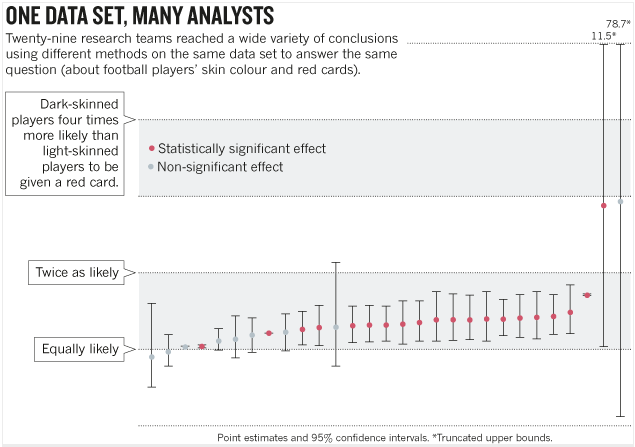
\includegraphics[width=\paperwidth]{../Images/Crowdsourcing2.PNG}
            };
        \end{tikzpicture}
     \end{frame}
}

\subsection*{Planes de Pre-Análisis}
\begin{frame}{Planes de Pre-Análisis}
\textbf{Explicación de la solución, de 3ie:}

``Un plan de pre-análisis (PAPs) is una descripción detallada de los análisis a ser conducidos. Esta descripción es escrita antes de los datos que contienen los impactos del programa bajo evaluación. Puede especificar las hipótesis a testear, como se construirán la variables, ecuaciones a estimar, controles a utilizar, y otros aspectos del análisis. Una función clave de los PAPs es incrementar la transparencia en investigación. Al especificar los detalles por adelantado antes de ver los resultados, el plan es un resguardo contra data mining y búsqueda de especificaciones. Se les recomienda a los investigadores que desarrollen y suban dichos planes junto con el registro de sus estudios. Sin embargo esto no es requisito para el registro de un estudio.''
study registration, but it is not required for registration.''
\end{frame}

\begin{frame}{Origenes: Regulacion Farmaceutica en USA}
``E9 Statistical Principles for Clinical Trials'' (1998)
\href{http://www.fda.gov/downloads/drugs/guidancecomplianceregulatoryinformation/guidances/ucm073137.pdf}{\beamergotobutton{Link}}

\S V Consideraciones en el Análisis de Datos
\begin{enumerate}[<.->]
\item Pre-especificación del análisis
\item Grupos de análisis
\item Tratamiento de NAs y valores extremos
\item Transformaciones a los datos
\item Estimación, intervalos de confianza, y testeo de hipótesis
\item Ajuste de significancia y niveles de confianza
\item Subgrupos, interacciones, y variables de control
\item Integridad de los datos y validez del software computacional
\end{enumerate}
\end{frame}

%%%%%%%%%%%%%%%%%%%%%%%%%%%%%%%%%%%%
%%%%%%%%%%%%%%%%%%%%%%%%%%%%%%%%%%%%
%%%%%%%%%%%%%%%%%%%%%%%%%%%%%%%%%%%%
\begin{frame}{Sugerencias de Glennerster, Takavarasha}
\textit{Running Randomized Evaluations}
\begin{enumerate}[<.->]
\def\labelenumi{\arabic{enumi}.}
\item
  como se van a medir los principales variables de resultado, 
\item
 Dentro de las variables de resultado: cuales son primarias, cuales secundarias?,
\item
composición exacta de toda la familia de tests utilizados en análisis de effectos promedios
  \begin{itemize}
  \item Explicación de efectos promedio , FWER, FDR en Anderson (\href{https://are.berkeley.edu/~mlanderson/pdf/Anderson\%202008a.pdf}{JASA 2008}).
  \end{itemize}
\item
  los subgrupos a ser analizados,
\item
la dirección esperada de los impactos si queremos usar test de una cola, y

\item
 la especificación primaria a ser utilizada en el análisis.
\end{enumerate}
\end{frame}

\begin{frame}{Sugerencias de McKenzie}
\href{http://blogs.worldbank.org/impactevaluations/a-pre-analysis-plan-checklist}{World Bank Development Impact Blog}

\begin{enumerate}[<.->]
\item
Descripción de la muestra a ser utilizada en el estudio
\item
 Fuentes de dato fundamentales
\item
Hipótesis a testear a través de la cadena causal
\item
Especificar como se van a construir la variables
\item
Especificar la ecuación donde se estimará el efecto del tratamiento 
\item
Cual es la estrategia para analizar multiples variables de resultados y múltiples test de hipótesis?
\item
Procedimiento a utilizar para enfrentar atrición en la muestra
\item
Qué hará el estudio en caso de limitada variación en las variables de resultados?
\item
Si hay un modelo a testear, este debe ser incluido
\item
No olvidar archivarlo (con una fecha estampada digitalmente)
\end{enumerate}
\end{frame}

%\begin{frame}{Simmons, Nelson, Simonsohn (2011)}
%\begin{enumerate}[<.->]
%\def\labelenumi{\arabic{enumi}.}
%\item
%  Authors must decide the rule for terminating data collection before data collection begins and report this rule in the article.
%\item
%  Authors must collect at least 20 observations per cell or else provide
%  a compelling cost-of-data-collection justification.
%\item
%  Authors must list all variables collected in a study.
%\item
%  Authors must report all experimental conditions, including failed
%  manipulations.
%\item
%  If observations are eliminated, authors must also report what the
%  statistical results are if those observations are included.
%\item
%  If an analysis includes a covariate, authors must report the
%  statistical results of the analysis without the covariate.
%\end{enumerate}
%\end{frame}

\begin{frame}{Ejemplos}

\begin{itemize}[<.->]
\item
J-PAL Registro de Hipotesis , ver \url{http://www.povertyactionlab.org/Hypothesis-Registry}

6 ejemplos de papers publicados:
\begin{itemize}
\item
 Sierra Leone CDD, Oregon Medicare, Turkey Job Training, El Salvador TOMS, dos en Indonesia (Olken et al.)
\end{itemize}
\item Psicología: \href{http://pss.sagepub.com/content/26/2/249}{Hawkins, Fitzgerald, Nosek---Riesgos de Concepción y Prejuicios}
\end{itemize} 
\vspace{0.25in}

Amplio rango de que es lo que se debe escribir exactamente y cuanto detalle incorporar en el PAP. En un nivel extremo el código estaría listo para ejecutar en cuanto lleguen los datos. .
\end{frame}

{ % all template changes are local to this group.
    \setbeamertemplate{navigation symbols}{}
    \begin{frame}[plain]
         \begin{tikzpicture}[remember picture,overlay]
            \node[at=(current page.center)] {
                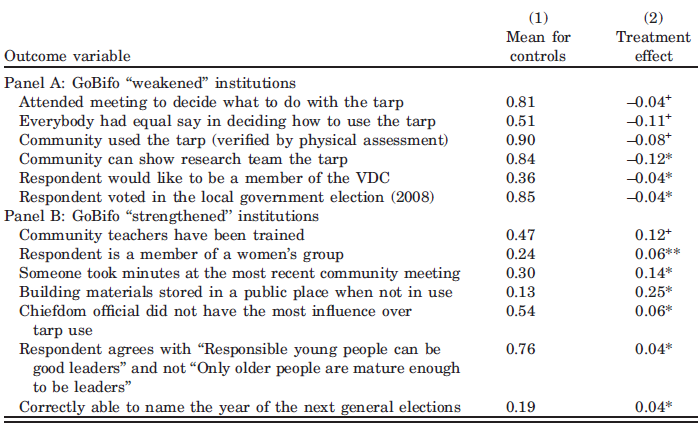
\includegraphics[width=\paperwidth]{../Images/GoBifo1.PNG}
            };
        \end{tikzpicture}
     \end{frame}
}

{ % all template changes are local to this group.
    \setbeamertemplate{navigation symbols}{}
    \begin{frame}[plain]
         \begin{tikzpicture}[remember picture,overlay]
            \node[at=(current page.center)] {
                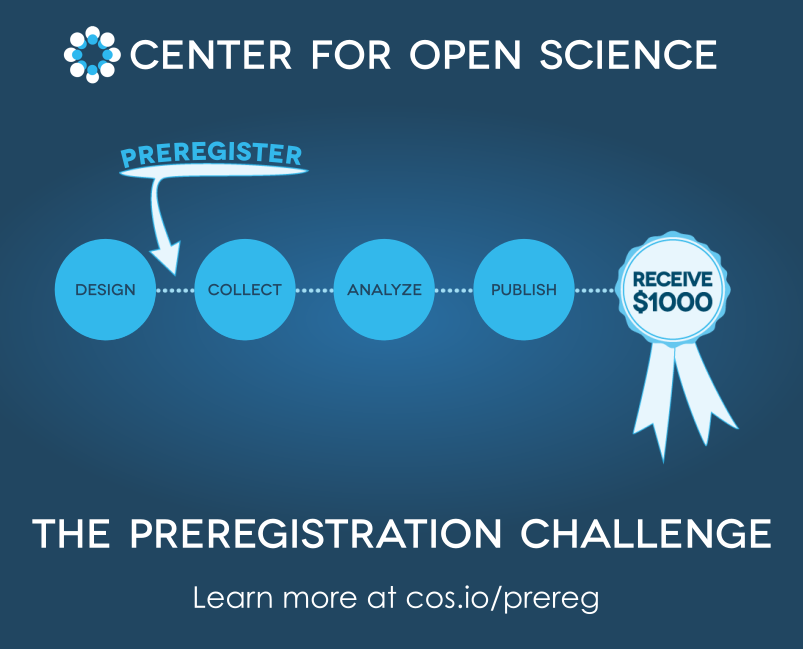
\includegraphics[width=\paperwidth]{../Images/preregchallenge.png}
            };
        \end{tikzpicture}
     \end{frame}
}
%%%%%%%%%%%%%%%%%%%%%%%%%%%%%%%%%%%%%%%%%%%%%%%%%%%%
\begin{frame}{PAP--Estudios Observacionales}
\begin{itemize}[<.->]
\item Actual debate en salud publica/epidemiologia.
\item Pre-especificar de manera verificable: dificil. pero no imposible.
\item Ejemplo: Datos generados periodicamente por el gobierno.
\item Ejemplo: Salario Mínimo (\href{http://onlinelibrary.wiley.com/doi/10.1111/0019-8676.00199/full}{Neumark 2001})
\end{itemize}
\end{frame}

{ % all template changes are local to this group.
    \setbeamertemplate{navigation symbols}{}
    \begin{frame}[plain]
         \begin{tikzpicture}[remember picture,overlay]
            \node[at=(current page.center)] {
                
\includegraphics[width=\paperwidth]{../Images/Neumark.PNG}
            };
        \end{tikzpicture}
     \end{frame}
}
%%%%%%%%%%%%%%%%%%%%%%%%%%%%%%%%%%%%%%%%%%%%%%%%%%%%%%%%%%%%%%%%%%%%
\section{Replicaciones}
\begin{frame}{Replicaciones}
\begin{enumerate}[<.->]
 \item El problema	\href{http://www.jstor.org/stable/1806061}{(JMCB Project)}
 \item Protocolo del proyecto, Estándares de publicación
 \item Organización del flujo de trabajo
 \item Compartir código y datos
\end{enumerate}
\end{frame}

 { % all template changes are local to this group.
    \setbeamertemplate{navigation symbols}{}
    \begin{frame}[plain, label=AEAreg]
         \begin{tikzpicture}[remember picture,overlay]
            \node[at=(current page.center)] {
                
\includegraphics[width=\paperwidth]{../Images/JMCB1.PNG}
            };
        \end{tikzpicture}
     \end{frame}
}

\subsection*{Protocolo del Proyecto, Estándares de Información}
\begin{frame}[<.->]{Protocolo del Proyecto, Estándares de Información}
Asegurar de que todo disponibilidad lo necesario para que otro investigador replique su investigación.
 \begin{itemize}
 \item Encuentre el estándar de información apropiado para su disciplina y sígalo: \url{http://www.equator-network.org}
\item Informe todos los detalles sobre la implementacion de un proyecto en un protocolo detallado: \url{http://www.spirit-statement.org}
\item Pautas Transparency and Openness Promotion (TOP): \url{http://cos.io/top}
\end{itemize}
\end{frame}

 { % all template changes are local to this group.
    \setbeamertemplate{navigation symbols}{}
    \begin{frame}[plain, label=AEAreg]
         \begin{tikzpicture}[remember picture,overlay]
            \node[at=(current page.center)] {
                
\includegraphics[width=\paperwidth]{../Images/TOPGuidelines.PNG}
            };
        \end{tikzpicture}
     \end{frame}
}

 \subsection*{Flujo de trabajo}
 \begin{frame}{Flujo de trabajo}
``Reproduciblidad es simplemente una colaboración con personas que aun no conoces, incluido tu mismo en una semana más'
---Philip Stark, UC Berkeley Statistics
\end{frame}

\begin{frame}{Flujo de trabajo}

 \begin{itemize}
 \item Sugerencias practicas sobre organización y programación
 \begin{itemize}[<.->]
 	\item Al realizar cambios a archivos que and sido compartidos/publicados, implica que debe renombrar el archivo.
 	\item Haga referencia a la version necesaria para ejecutar funciones.
 	\item Long (2008) \textit{The Workflow of Data Analysis Using Stata}
  \end{itemize}
 \item Programación Literaria: comentario extensivo en el código, apuntando a que sea legible por humanos
 \item Control de Versiones
 \item Documentos Dinámicos
\end{itemize}
\end{frame}

\subsection*{Control de Versiones}
\begin{frame}{Control de Versiones}
\begin{itemize}[<.->]
\item
Utilizar control de versiones puede ayudar a hacer su trabajo más reproducible.

\item
Qué es Control de Versiones?

\begin{quote}
Control de versiones es un sistema que registra cambios a uno o varios archivos en el tiempo, de forma tal que versiones especifica pueden ser recuperados más adelante.
\end{quote}
--Git, \href{https://git-scm.com/book/en/v2/Getting-Started-About-Version-Control}{About Version Control}
%\item Distributed Version Control Systems (DCVS) let multiple users control the same files in this manner.
\end{itemize}
\end{frame}

 { % all template changes are local to this group.
    \setbeamertemplate{navigation symbols}{}
    \begin{frame}[plain, label=AEAreg]
         \begin{tikzpicture}[remember picture,overlay]
            \node[at=(current page.center)] {
                
\includegraphics[height=\paperheight]{../Images/github-logo-transparent.JPG}
            };
        \end{tikzpicture}
     \end{frame}

 % all template changes are local to this group.
    \setbeamertemplate{navigation symbols}{}
    \begin{frame}[plain]
         \begin{tikzpicture}[remember picture,overlay]
            \node[at=(current page.center)] {
                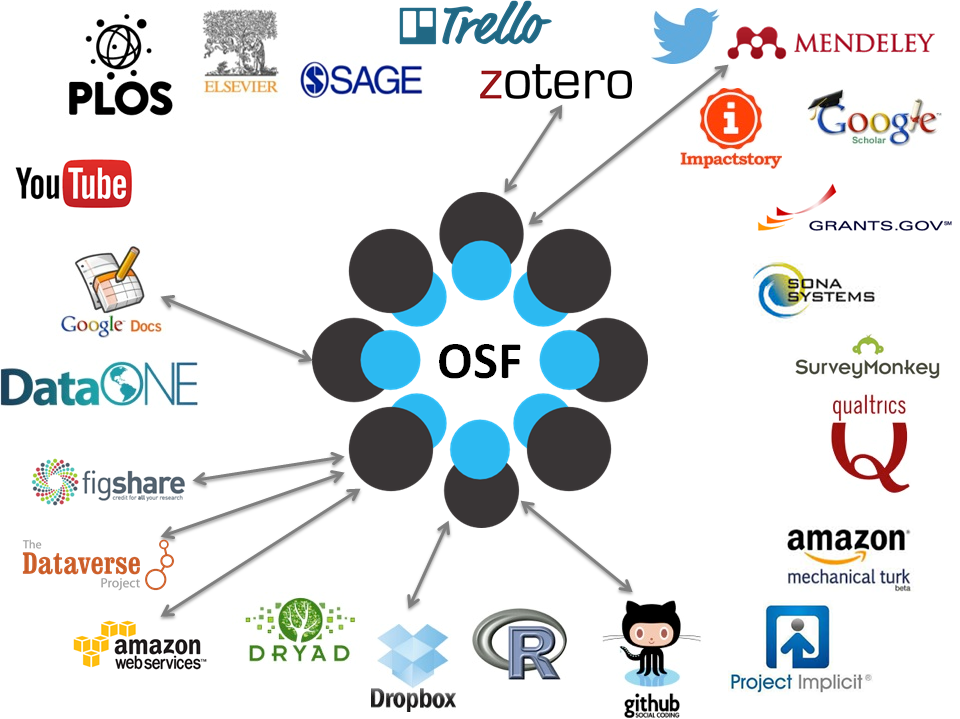
\includegraphics[width=\paperwidth]{../Images/OSFnow.PNG}
            };
        \end{tikzpicture}
     \end{frame}

% all template changes are local to this group.
    \setbeamertemplate{navigation symbols}{}
    \begin{frame}[plain]
         \begin{tikzpicture}[remember picture,overlay]
            \node[at=(current page.center)] {
                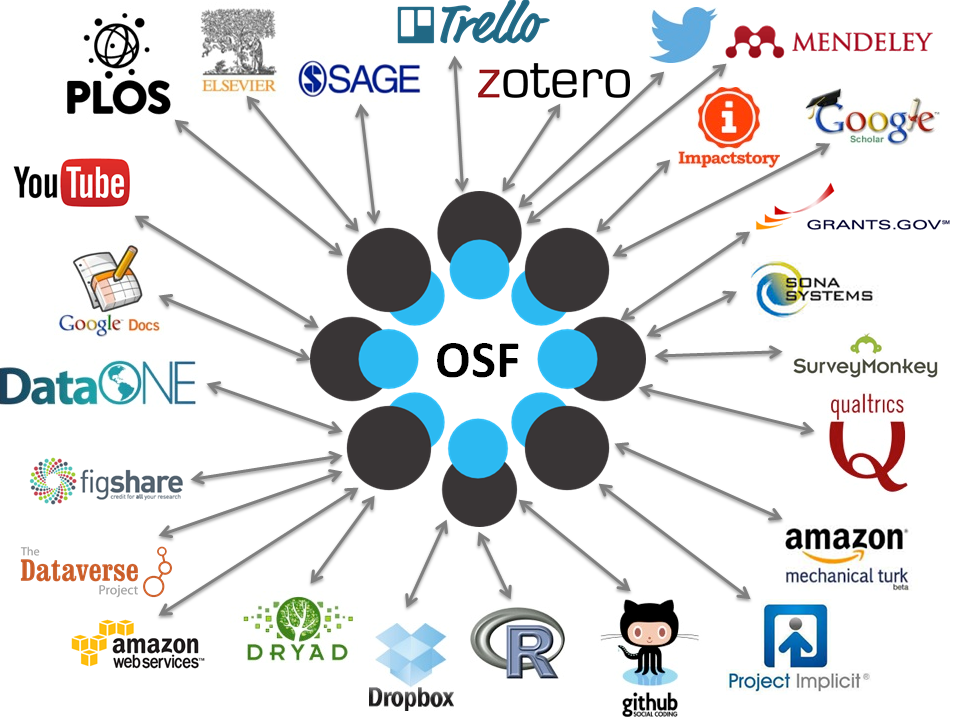
\includegraphics[width=\paperwidth]{../Images/OSFsoon.PNG}
            };
        \end{tikzpicture}
     \end{frame}

}


\begin{frame}{Documentos Dinámicos}

Meta aspiracional: Escriba su código y su paper en el mismo archivo. De esta forma se minimiza la perdida de información y se eliminan errores de copiar/pegar.

\medskip
Establecido en R/Python y comenzando en Stata.
\begin{itemize}[<.->]
\item Incluye tablas dentro del archivo, en lugar de copiar-pegar-formatear elementos estáticos
\item Todas las cifras dentro del texto también son calculadas de manera dimanica, eliminando la necesidad de tipeo de cifras manualmente.
\item Cifras y tablas se actualizan automáticamente.
\item El paper completo es (re)producido con uno o dos clicks
\end{itemize} 
\end{frame}


 { % all template changes are local to this group.
    \setbeamertemplate{navigation symbols}{}
    \begin{frame}[plain, label=AEAreg]
         \begin{tikzpicture}[remember picture,overlay]
            \node[at=(current page.center)] {
                
\includegraphics[height=\paperheight]{../Images/jupyter.png}
            };
        \end{tikzpicture}
     \end{frame}
}
 { % all template changes are local to this group.
    \setbeamertemplate{navigation symbols}{}
    \begin{frame}[plain, label=AEAreg]
         \begin{tikzpicture}[remember picture,overlay]
            \node[at=(current page.center)] {
                
\includegraphics[width=\paperwidth]{../Images/RStudio-Logo-Blue-Gradient.png}
            };
        \end{tikzpicture}
     \end{frame}
}

\subsection*{Compartiendo lo Datos}
\begin{frame}{Compartiendo lo Datos}
Publique su codigo y sus datos en un repositorio publico de confianza.\begin{itemize}[<.->]
\item
Encuentre el repositorio apropiado: \url{http://www.re3data.org/}
\item
Los repositorios están diseñados para durar más que su website.
\item
También están diseñados para facilitar la búsqueda por parte de otros investigadores.
\item
Los repositorios guardan sus datos en formatos publicos que evitan obsolescencia en el tiempo.
\end{itemize}
\end{frame}

\section{Conclusión}
\begin{frame}{Conclusión}
OK, estoy convencido. Como puedo implementar esto en mi propia investigación?

\begin{itemize}[<.->]
\item Tomen nuestro MOOC (E. Miguel).\href{https://www.futurelearn.com/courses/open-social-science-research}{\beamergotobutton{Link}}
\item Suscribance al blog \& E-mail de BITSS \href{https://bitss.org/blog}{\beamergotobutton{Link}}
\item Apliquen a nuestro summer institute: RT2. \href{http://www.bitss.org/events/summer-institute/}{\beamergotobutton{Link}}
\item Apliquen a nuestros fondos de investigacion SSMART (fondos adicionales para investigadores de paises en desarrollo). \href{http://www.bitss.org/ssmart-grants/}{\beamergotobutton{Link}}
\item Apliquen al premio Leamer-Rosenthal. \href{http://www.bitss.org/lr-prizes/}{\beamergotobutton{Link}}
\item Revisen nuestra pagina de recursos. \href{http://www.bitss.org/resource-tag/education/}{\beamergotobutton{Link}}
\item Interesado en incluir parte de estas practicas en el análisis de políticas publicas? Hablen conmigo! \href{mailto:fhoces@berkeley.edu}{fhoces@berkeley.edu}

\end{itemize}
\end{frame}

\begin{frame}{RT2}
Tres días de entrenamiento. Evento anual que alterna entre Berkeley y fuera de USA (Londres fue hace dos semanas)
'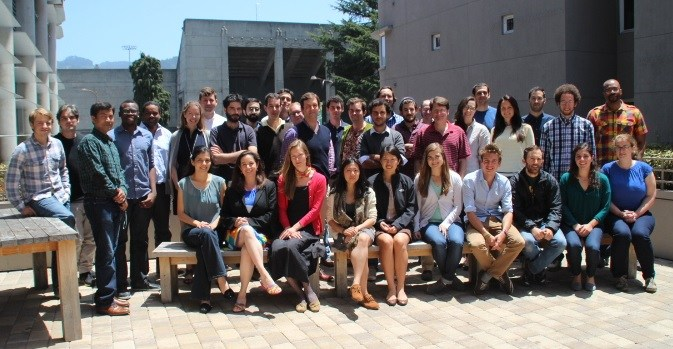
\includegraphics[width=4in]{../Images/bitss-2014-cohort2.jpg}
\end{frame}

\begin{frame}{Fondos SSMART}
Fondos de hasta \$30,000 para financiar investigación en transparencia:
\begin{itemize}[<.->]
\item Desarrollo de nuevas metodologías
\item Nuevas herramientas y usos de meta-análisis
\item Investigación sobre comportamiento de investigadores y adopción de nuevas normas
\end{itemize}
Financiamiento extra para investigadores de paises en desarrollo.

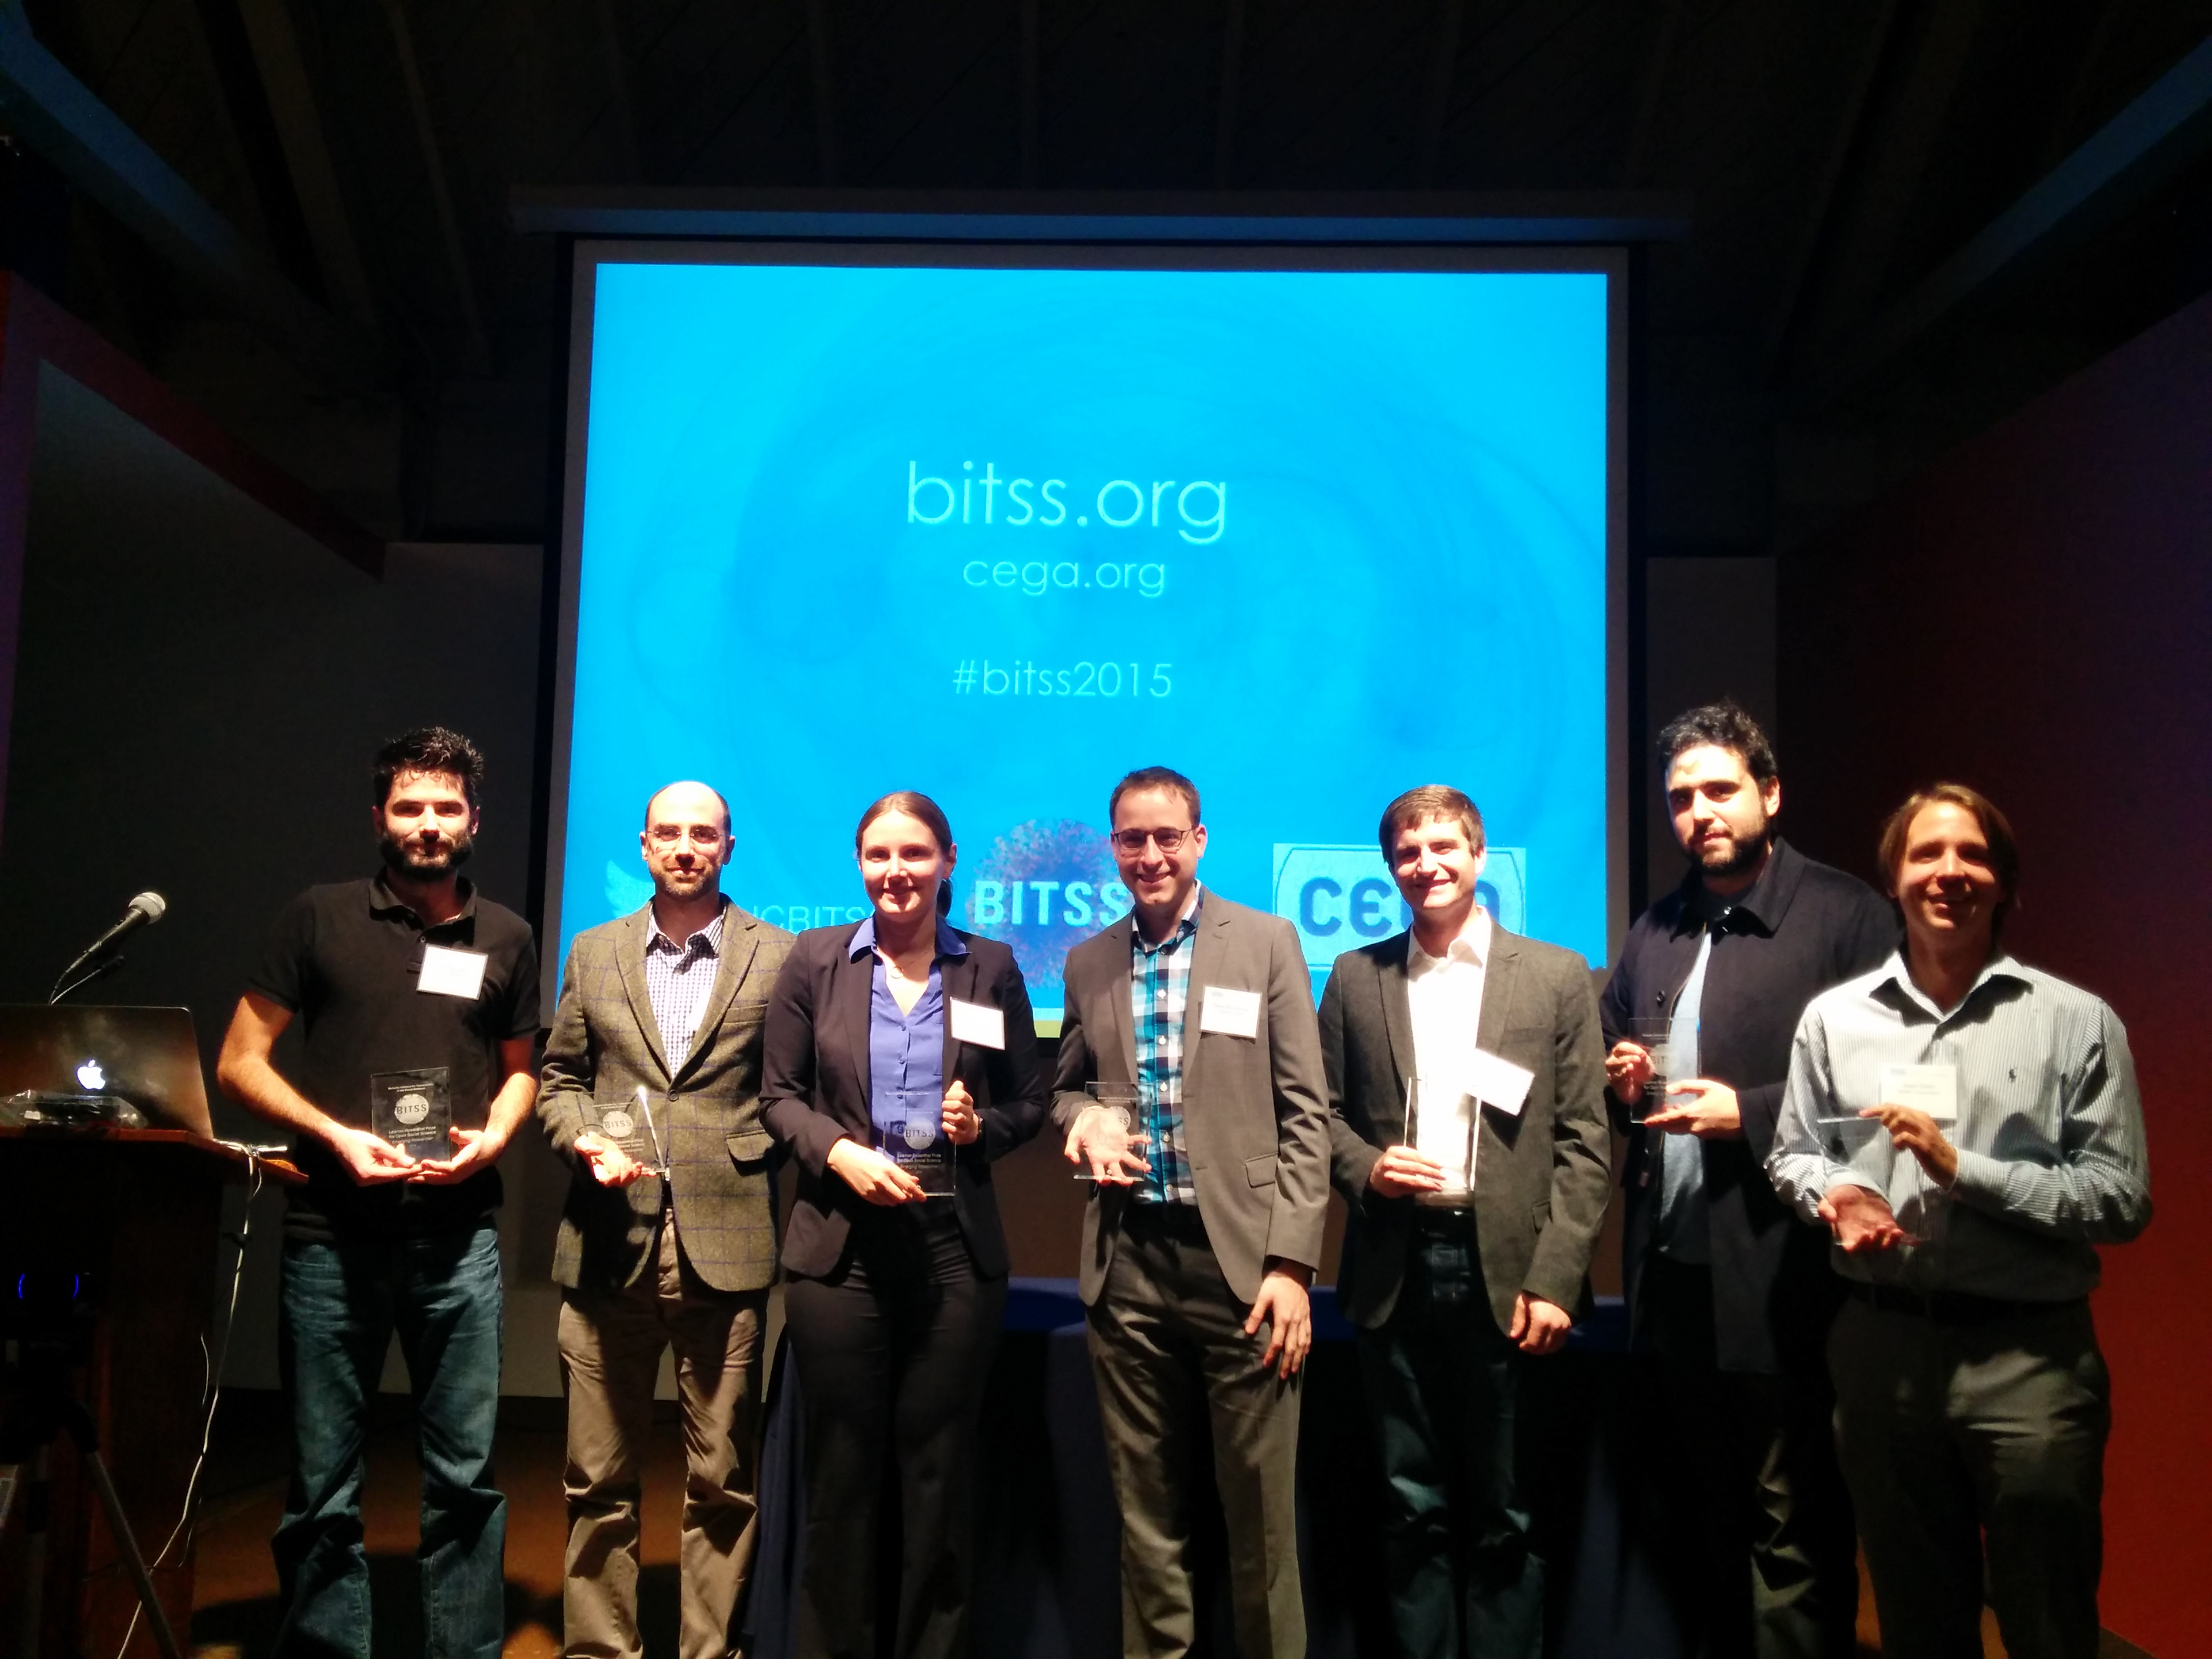
\includegraphics[width=2.5in]{../Images/LRwinners.jpg}
\end{frame}

\begin{frame}{Premio Leamer-Rosenthal}
Reconocimiento a investigadores que han completado estudios en/sobre transparencia y reproducibilidad en ciencias sociales,
Ejemplos:
\begin{itemize}[<.->]
\item Psicología
\item Ciencias Políticas
\item Economía
\end{itemize}
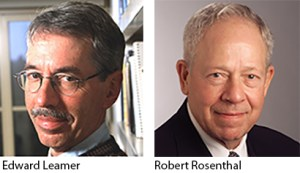
\includegraphics[width=2.5in]{../Images/leamer1-zoomed33.jpg}
\end{frame}


\begin{frame}
\begin{center}
Preguntas?
\vspace{0.5in}


\Huge{Muchas Gracias}
\end{center}
\end{frame}

\end{document}

